\usetikzlibrary{calc}
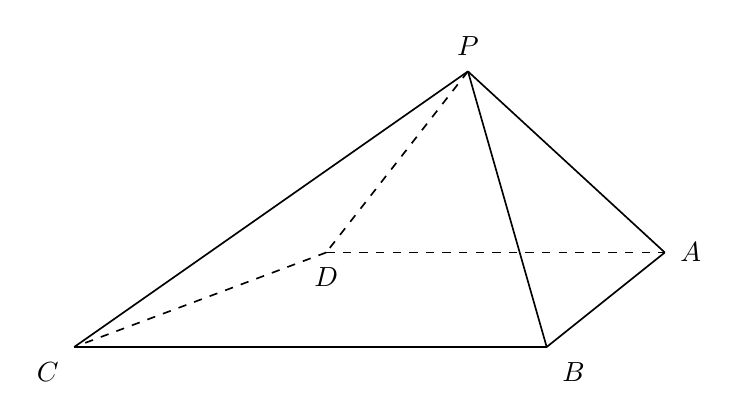
\begin{tikzpicture}[line width=0.6pt, font=\normalsize]
\coordinate (C) at (0.0,0.0);
\coordinate (B) at (6.0,0.0);
\coordinate (A) at (7.5,1.2);
\coordinate (D) at (3.2,1.2);
\coordinate (P) at (5.0,3.5);
\draw[solid] (C) -- (B) -- (A);
\draw[solid] (P) -- (C);
\draw[solid] (P) -- (B);
\draw[solid] (P) -- (A);
\draw[dashed] (D) -- (C);
\draw[dashed] (D) -- (A);
\draw[dashed] (P) -- (D);
\node[below left=2pt] at (C) {$C$};
\node[below right=2pt] at (B) {$B$};
\node[right=2pt] at (A) {$A$};
\node[below=2pt] at (D) {$D$};
\node[above=2pt] at (P) {$P$};
\end{tikzpicture}
